\documentclass{article}

% packages
\usepackage{amsmath, amsthm, thmtools, amsfonts, amssymb, luacode, catchfile, tikzducks, hyperref, ifthen}
\ifcsname c@kobocompile\endcsname
	\usepackage[a5paper, total={1072pt, 1448pt}, margin=10pt, includeheadfoot]{geometry} % set page margins
\else
	\usepackage[a4paper, margin=50pt, includeheadfoot]{geometry}
\fi
\usepackage[shortlabels]{enumitem}
\usepackage[skip=3pt, indent=0pt]{parskip}

% language
\usepackage[bidi=basic, layout=tabular, provide=*]{babel}
\ifcsname c@english\endcsname
	\babelprovide[main, import]{english}
\else
	\babelprovide[main, import]{hebrew}
	\babelprovide{rl}
\fi
%\babelfont{rm}{Libertinus Serif}
\babelfont{rm}[Renderer=Harfbuzz]{Libertinus Serif}
\babelfont{sf}{Libertinus Sans}
\babelfont{tt}{Libertinus Mono}

% style
\AddToHook{cmd/section/before}{\clearpage}	% Add line break before section
\linespread{1.3}
\setcounter{secnumdepth}{0}		% Remove default number tags from sections, this won't do well with theorems
\AtBeginDocument{\setlength{\belowdisplayskip}{3pt}}
\AtBeginDocument{\setlength{\abovedisplayskip}{3pt}}
\graphicspath{ {../images/} }

% operators
\DeclareMathOperator\cis{cis}
\DeclareMathOperator\Sp{Sp}
\DeclareMathOperator\tr{tr}
\DeclareMathOperator\im{Im}
\DeclareMathOperator\re{Re}
\DeclareMathOperator\diag{diag}
\DeclareMathOperator*\lowlim{\underline{lim}}
\DeclareMathOperator*\uplim{\overline{lim}}
\DeclareMathOperator\rng{rng}
\DeclareMathOperator\Sym{Sym}
\DeclareMathOperator\Arg{Arg}
\DeclareMathOperator\Log{Log}
\DeclareMathOperator\dom{dom}
\DeclareMathOperator\supp{Supp}
\DeclareMathOperator\var{Var}
\DeclareMathOperator\cov{Cov}

% commands
%\renewcommand\qedsymbol{\textbf{מש''ל}}
%\renewcommand\qedsymbol{\fbox{\emoji{lizard}}}
\newcommand{\Aa}[0]{\mathcal{A}}
\newcommand{\Bb}[0]{\mathcal{B}}
\newcommand{\CC}[0]{\mathbb{C}}
\newcommand{\Cc}[0]{\mathcal{C}}
\newcommand{\EE}[0]{\mathbb{E}}
\newcommand{\FF}[0]{\mathbb{F}}
\newcommand{\Ff}[0]{\mathcal{F}}
\newcommand{\Ii}[0]{\mathcal{I}}
\newcommand{\Gg}[0]{\mathcal{G}}
\newcommand{\Ll}[0]{\mathcal{L}}
\newcommand{\Mm}[0]{\mathcal{M}}
\newcommand{\NN}[0]{\mathbb{N}}
\newcommand{\Nn}[0]{\mathcal{N}}
\newcommand{\PP}[0]{\mathbb{P}}
\newcommand{\Pp}[0]{\mathcal{P}}
\newcommand{\QQ}[0]{\mathbb{Q}}
\newcommand{\RR}[0]{\mathbb{R}}
\newcommand{\Rr}[0]{\mathcal{R}}
\newcommand{\Ss}[0]{\mathcal{S}}
\newcommand{\TT}[0]{\mathbb{T}}
\newcommand{\Uu}[0]{\mathcal{U}}
\newcommand{\Vv}[0]{\mathcal{V}}
\newcommand{\Ww}[0]{\mathcal{W}}
\newcommand{\ZZ}[0]{\mathbb{Z}}
\newcommand{\acts}[0]{\circlearrowright}
\newcommand{\explain}[2] {
	\begin{flalign*}
		 && \text{#2} && \text{#1}
	\end{flalign*}
}
\newcommand{\maketitleprint}[0]{ \begin{center}
	%\begin{tikzpicture}[scale=3]
	%	\duck[graduate=gray!20!black, tassel=red!70!black]
	%\end{tikzpicture}	
	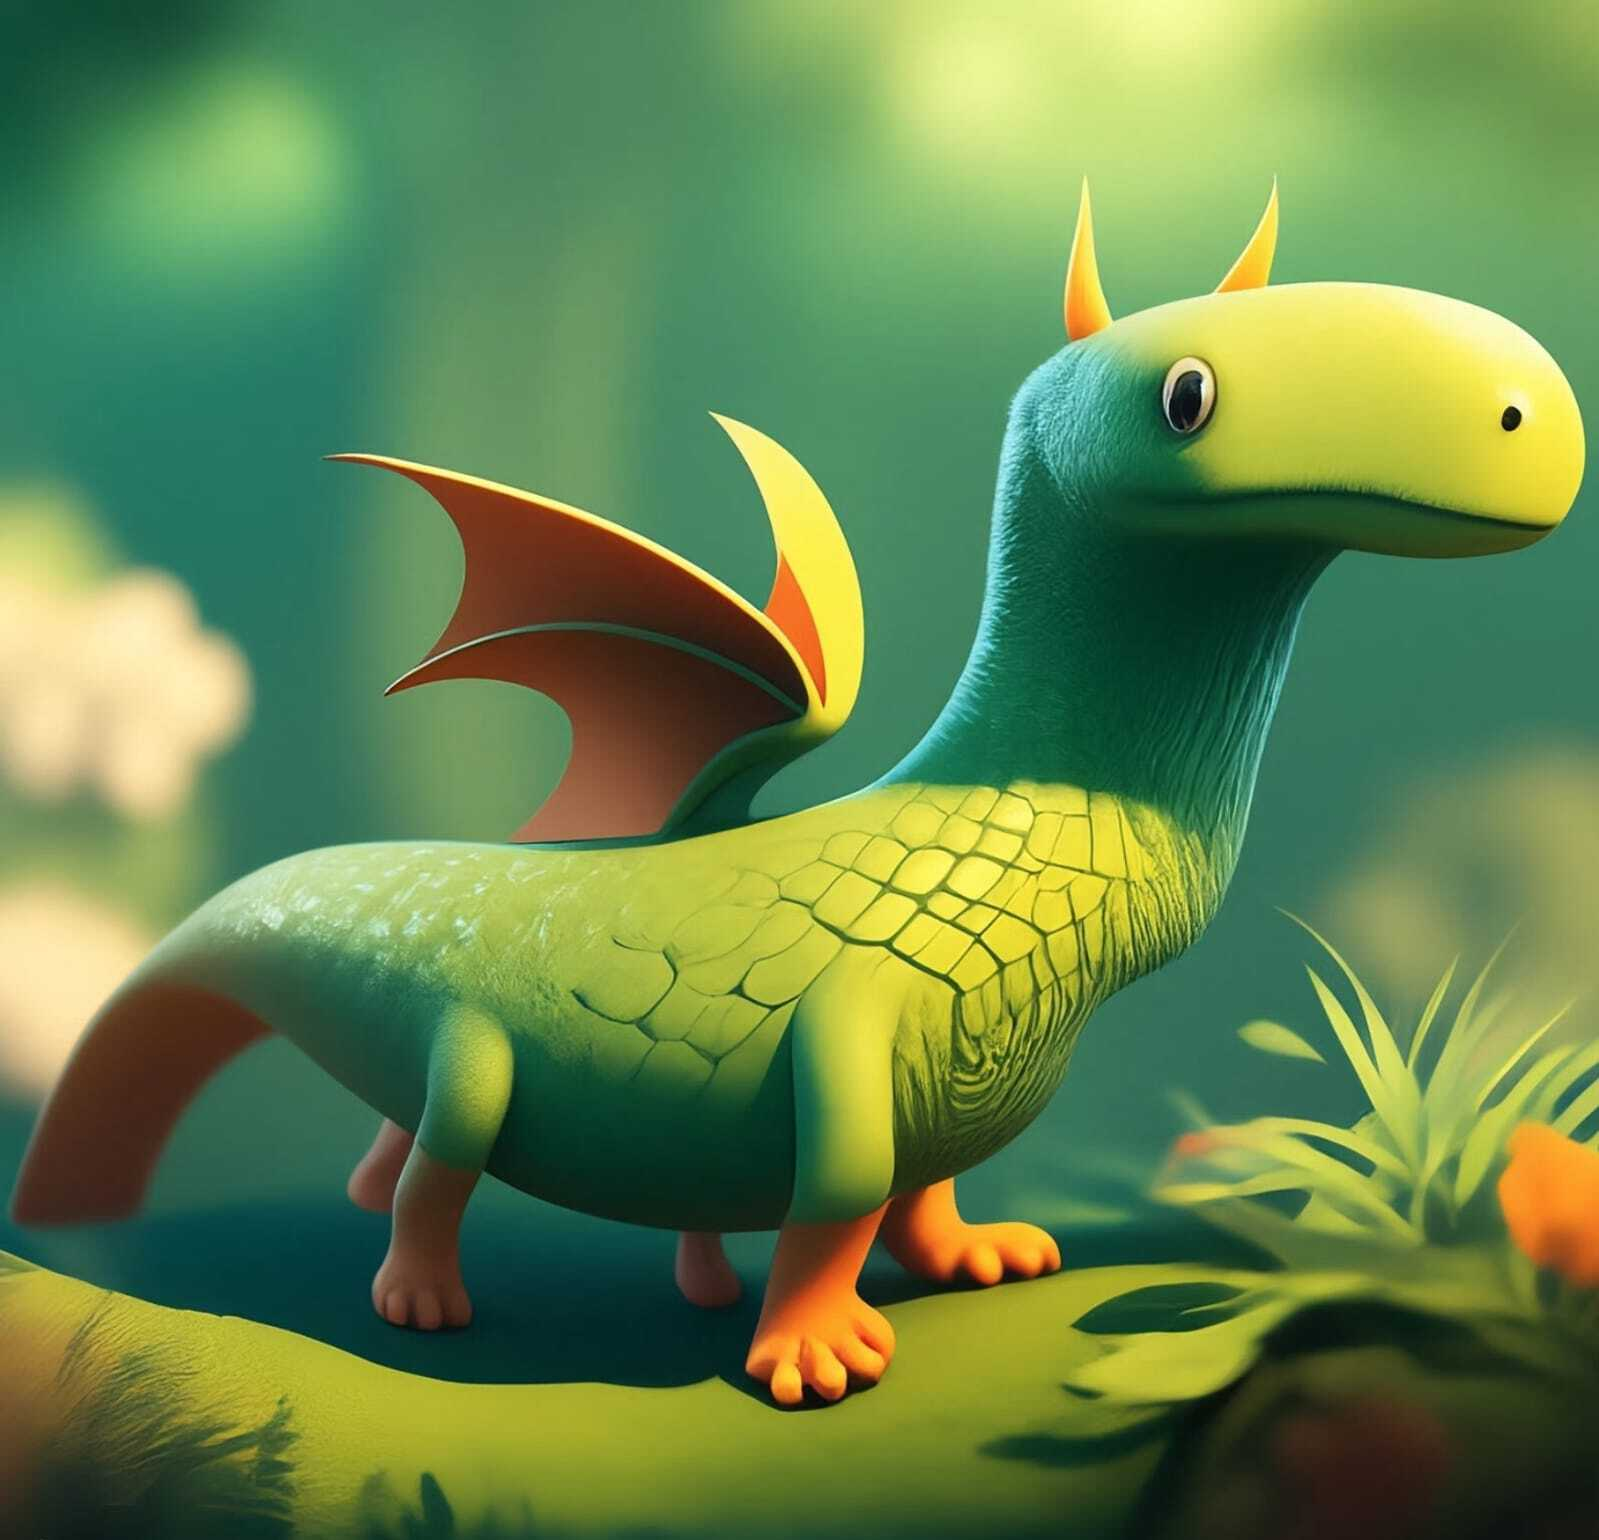
\includegraphics[width=6cm]{cover}
\end{center}
}

% theorem commands
\newtheoremstyle{c_remark}
	{}	% Space above
	{}	% Space below
	{}% Body font
	{}	% Indent amount
	{\bfseries}	% Theorem head font
	{}	% Punctuation after theorem head
	{.5em}	% Space after theorem head
	{\thmname{#1}\thmnumber{ #2}\thmnote{ \normalfont{\text{(#3)}}}}	% head content
\newtheoremstyle{c_definition}
	{3pt}	% Space above
	{3pt}	% Space below
	{}% Body font
	{}	% Indent amount
	{\bfseries}	% Theorem head font
	{}	% Punctuation after theorem head
	{.5em}	% Space after theorem head
	{\thmname{#1}\thmnumber{ #2}\thmnote{ \normalfont{\text{(#3)}}}}	% head content
\newtheoremstyle{c_plain}
	{3pt}	% Space above
	{3pt}	% Space below
	{\itshape}% Body font
	{}	% Indent amount
	{\bfseries}	% Theorem head font
	{}	% Punctuation after theorem head
	{.5em}	% Space after theorem head
	{\thmname{#1}\thmnumber{ #2}\thmnote{ \text{(#3)}}}	% head content

\ifcsname c@english\endcsname
	\theoremstyle{plain}
	\newtheorem{theorem}{Theorem}[section]
	\newtheorem{lemma}[theorem]{Lemma}
	\newtheorem{proposition}[theorem]{Proposition}
	\newtheorem*{proposition*}{Proposition}
	%\newtheorem{corollary}[theorem]{אין חלופה עברית}

	\theoremstyle{definition}
	\newtheorem{definition}[theorem]{Definition}
	\newtheorem*{definition*}{Definition}
	\newtheorem{example}{Example}[section]
	\newtheorem{exercise}{Exercise}[section]

	\theoremstyle{remark}
	\newtheorem*{remark}{Remark}
	\newtheorem*{solution}{Solution}
	\newtheorem{conclusion}[theorem]{Conclusion}
	\newtheorem{notation}[theorem]{Notation}
\else
	\theoremstyle{c_plain}
	\newtheorem{theorem}{משפט}[section]
	\newtheorem{lemma}[theorem]{למה}
	\newtheorem{proposition}[theorem]{טענה}
	\newtheorem*{proposition*}{טענה}
	%\newtheorem{corollary}[theorem]{אין חלופה עברית}

	\theoremstyle{c_definition}
	\newtheorem{definition}[theorem]{הגדרה}
	\newtheorem*{definition*}{הגדרה}
	\newtheorem{example}{דוגמה}[section]
	\newtheorem{exercise}{תרגיל}[section]

	\theoremstyle{c_remark}
	\newtheorem*{remark}{הערה}
	\newtheorem*{solution}{פתרון}
	\newtheorem{conclusion}[theorem]{מסקנה}
	\newtheorem{notation}[theorem]{סימון}
\fi

% Questions related commands
\newcounter{question}
\setcounter{question}{1}
\newcounter{sub_question}
\setcounter{sub_question}{1}

\ifcsname c@english\endcsname
	\newcommand{\question}[1][0]{
		\ifthenelse{#1 = 0}{}{\setcounter{question}{#1}}
		\section{Question \arabic{question}}
		\addtocounter{question}{1}
		\setcounter{sub_question}{1}
	}

	\newcommand{\subquestion}[1][0]{
		\ifthenelse{#1 = 0}{}{\setcounter{sub_question}{#1}}
		\subsection{Part \alph{sub_question}}
		\addtocounter{sub_question}{1}
	}
\else
	\newcommand{\question}[1][0]{
		\ifthenelse{#1 = 0}{}{\setcounter{question}{#1}}
		\section{שאלה \arabic{question}}
		\addtocounter{question}{1}
		\setcounter{sub_question}{1}
	}

	\newcommand{\subquestion}[1][0]{
		\ifthenelse{#1 = 0}{}{\setcounter{sub_question}{#1}}
		\subsection{סעיף \localecounter{letters.gershayim}{sub_question}}
		\addtocounter{sub_question}{1}
	}
\fi

% import lua and start of document
\directlua{common = require ('../common')}

\GetEnv{AUTHOR}

% headers
\author{\AUTHOR}
\date\today

\title{תורת המודלים 1 --- סיכום}
\setcounter{secnumdepth}{2}

\usepackage{fancyhdr}
\pagestyle{fancy}
\renewcommand{\headrulewidth}{0pt}

\begin{document}
\maketitle
\maketitleprint[purple]

\tableofcontents

\setcounter{section}{-1}
\section{שיעור הכנה}
\subsection{מעט תורת הקבוצות}
\begin{definition}[מונה]
	סודר $\alpha$ נקרא מונה אם לכל $\beta < \alpha$ אין העתקה על $f : \beta \to \alpha$ (שקול לאי־קיום פונקציה חד־חד ערכית).
\end{definition}
\begin{example}
	כל הסודרים הסופיים הם מונים, וכך גם $\omega$.
\end{example}
\begin{example} 
	$\omega + 1, \omega + 2, \ldots$ הם לא מונים כי נוכל לבנות פונקציה $f : \omega + n \to \omega$ חד־חד ערכית.
\end{example}
נגדיר לדוגמה גם את $\omega_1 = \aleph_1$ להיות המונה הבא אחרי $\omega$.
\begin{theorem}[אי־חסימות מונים]
	לכל מונה $\kappa$ יש מונה $\mu > \kappa$.
\end{theorem}
\begin{proof}
	בהנחת אקסיומת הבחירה נסדר את $\Pp(\kappa)$ בסדר טוב בטיפוס סדר $\alpha$.
	אז אין העתקה על מ־$\kappa$ ל־$\alpha$.
	יהי $\mu > 0$ הסודר הראשון כך שאין העתקה על מ־$\kappa$ ל־$\mu$ ונטען כי $\mu$ מונה. \\
	אם $\mu$ איננו מונה, אז יש $\beta < \mu$ והעתקה חד־חד ערכית ועל $g : \alpha \to \beta$, והרכבת הפונקציות מספקת סתירה.
\end{proof}
ישנה גם הוכחה ללא אקסיומת הבחירה אבל לא נביא אותה בסיכום זה.
\begin{definition}[מונה עוקב]
	המונה הראשון שגדול ממונה $\kappa$ נקרא העוקב של $\kappa$ ומסומן $\kappa^+$.
\end{definition}
\begin{remark}
	אם $A$ קבוצת מונים, אז גם $\bigcup A$ מונה.
\end{remark}
אנו יכולים לבחון את $\aleph_0 = \omega$ וכן את $\aleph_1 = \aleph_0^+$ וכן הלאה, ולבסוף נוכל להגדיר גם את $\aleph_{\omega} = \sup\{ \aleph_n \mid n < \omega \}$, וכן $\aleph_{\omega + 1} = \aleph_{\omega}^+$.
\begin{theorem}[היררכיית אלף]
	כל מונה הוא $\aleph_{\alpha}$ עבור איזשהו סודר $\alpha$.
\end{theorem}
\begin{proof}
	נניח ש־$\kappa$ מונה, אז $\kappa \le \aleph_{\kappa}$ (ניתן להוכחה באינדוקציה טרנספיניטית).
	לכן קיים $\gamma$ הסודר הראשון כך ש־$\kappa \le \aleph_{\gamma}$.
	אם $\kappa < \aleph_{\gamma}$ אז נחלק למקרים.
	אם $\gamma = \delta + 1$ אז $\aleph_{\gamma} = \aleph_{\delta}^+$ אבל $\aleph_{\delta} < \kappa < \aleph_{\delta + 1}$ ואז $\kappa = \aleph_{\delta}$.
	אם $\gamma$ גבולי, אז $\aleph_{\gamma} = \sup\{ aleph_{\beta} \mid \beta < \gamma \}$ ולכן יש $\beta < \gamma$ כך ש־$\kappa \le \aleph_{\beta}$ כסתירה.
	לכן נסיק ש־$\kappa = \aleph_{\gamma}$.
\end{proof}
\begin{corollary}
	אם $\alpha$ סודר ו־$\kappa \le \alpha$ מונה ומקסימלי מבין המונים $\le \alpha$, אז $|\alpha| = |\kappa| = \kappa$.
\end{corollary}
\begin{proof}
	באינדוקציה.
\end{proof}
\begin{definition}[מונה סדיר]
	מונה אינסופי $\kappa$ יקרא סדיר (regular) אם אין $\mu < \kappa$ ופונקציה $f : \mu \to \kappa$ כך ש־$\sup \rng f = \kappa$.
\end{definition}
ניצוק תוכן להגדרה זו.
\begin{proposition}
	מונה $\kappa$ הוא סדיר אם ורק אם אין פירוק של $\kappa$ כאיחוד של קבוצות $\kappa = \bigcup \{ A_i \mid i < \mu \}$ כך ש־$\mu < \kappa$ וכן $|A_i| < \kappa$.
\end{proposition}
\begin{example}
	$\omega$ הוא סדיר, תחת אקסיומת הבחירה גם $\omega_1$ הוא סדיר.
	נניח ש־$f : \mu \to \omega_1$ עבור $\mu < \omega_1$ וכן $\sup \rng f = \bigcup \{ f(\delta) \mid \delta < \mu \}$ כאשר $f(\delta)$ בן־מניה.
	אבל מאקסיומת הבחירה איחוד בן־מניה של קבוצות בנות־מניה הוא גם בן־מניה.
\end{example}
\begin{definition}
	מונה $\kappa$ יקרא חריג אם הוא אינסופי ואינו סדיר.
\end{definition}
\begin{example}
	$\aleph_{\omega}$ הוא מונה חריג.
	נגדיר $f(n) = \omega_n = \aleph_n$ כאשר $f : \omega \to \aleph_{\omega}$.
\end{example}
\begin{proposition}
	לכל מונה אינסופי $\kappa$ מתקיים $|\kappa| = |\kappa \times \kappa|$.
\end{proposition}
\begin{proof}
	נספק סקיצה כללית.
	נוכיח באינדוקציה על מונים אינסופיים. \\
	ל־$\omega$ זה ידוע וקל. \\
	נניח ש־$\kappa$ מונה כך שהטענה נכונה למונים קטנים ממנו.
	נגדיר סדר טוב על $\kappa \times \kappa$ באופן הבא,
	\begin{align*}
		\langle \alpha, \beta \rangle \le (\gamma, \delta)
		\iff & (\max\{ \alpha, \beta \} < \max\{ \gamma, \delta \}) \\
		\lor & (\max\{ \alpha, \beta \} = \max\{ \gamma, \delta \} \land \alpha < \gamma) \\
		\lor & (\max\{ \alpha, \beta \} = \max\{ \gamma, \delta \} \land \alpha = \gamma \land \beta \le \delta)
	\end{align*}
	נשים לב כי מתחת ל־$\langle \alpha, \beta \rangle$ יש פחות מ־$\kappa$ איברים,
	\[
		\le |\alpha + 1| \times |\beta + 1|
		\le |\mu_1 \times \mu_2|
		\le |\mu \times \mu|
		< \kappa
	\]
	עבור $\mu = \max(\mu_1, \mu_2) < \kappa$.
	הסדר שהגדרנו איזומורפי לסודר $\delta \le \kappa$ ולכן $\kappa \le |\kappa \times \kappa| \le \kappa$.
\end{proof}
\begin{corollary}
	לכל מונה $\kappa$ מתקיים $|\kappa^{< \omega}| = \kappa$.
\end{corollary}
\begin{theorem}[מונה עוקב הוא סדיר]
	אם $\kappa$ מונה אז $\kappa^+$ מונה סדיר.
\end{theorem}
\begin{proof}
	נניח בשלילה שלא ותהי $f : \mu \to \kappa^+$ כך ש־$\bigcup \{ f(\alpha) \mid \alpha < \mu \} = \kappa^+$. \\
	באמצעות בחירה לכל $\alpha$ נבחר $H_{\alpha} : \kappa \twoheadrightarrow f(\alpha) + 1$ וכן $H(\alpha, \beta) = H_{\alpha}(\beta)$ עבור $H : \mu \times \kappa \twoheadrightarrow \kappa^+$, וזו כמובן סתירה.
\end{proof}

\section{שיעור 1 --- 19.10.2025}
\subsection{רקע}
שעת קבלה בימי ראשון בשתיים־עשרה.
יהיו כשישה תרגילים ומטלה מסכמת.
תורת המודלים היא תחום בלוגיקה שעוסקת בניתוח של תורות ושל מודלים המתקבלים מהם.
נראה דוגמה למשפט שנובע מתחום זה.
\begin{example}
	משפט אקס־גרוטנדיק, הגורס כי אם פונקציה $f : \CC^n \to \CC^n$ כך שכל קורדינטה שלה היא פולינום ב־$n$ משתנים.
	נניח ש־$f$ חד־חד ערכית, אז $f$ היא גם על.
\end{example}
זהו משפט מוזר מאוד ומפתיע.
הדרך להוכיח אותו היא כזו,
נניח שיש לנו סדרה של פולינומים כך שהם חד־חד ערכיים ולא על, אז הכישלון שנקבל הוא על־ידי פסוק מסדר ראשון בשפת תורת החוגים $\varphi$ כך ש־$\CC \models \varphi$.
\[
	\exists a_0, \ldots, \exists a_{N}\ \forall \bar{x} \forall \bar{y}\ (a_0 x_0 \cdots = a_0 y_0 \cdots) \to \bar{x} = \bar{y}
	\land \exists \bar{z} \forall \bar{x} \lnot \bigwedge_{i < N} a_0 \bar{x} = z_i
\]
נבחין כי מתקיימת העובדה שנוכיח בהמשך,
\begin{remark}
	התורה של שדה סגור אלגברית ממציין נתון היא שלמה.
	בפרט כל שדה סגור אלגברית ממציין 0 מקיים את $\varphi$.
\end{remark}
מההערה ושלמות נסיק שכל שדה מספיק סגור אלגברית ממימד מספיק גדול מקיים את $\varphi$.
בפרט ל־$p$ ראשוני מספיק גדול $\overline{\FF}_p \models \varphi$.
נסתכל על מקדמים של הפולינום הבעייתי $a_0, \ldots, a_{N}$ ונקבל שהם שייכים ל־$\FF_p[a_0, \ldots, a_{N}] = \tilde{\FF}$ שדה סופי כלשהו.
נניח ש־$z_{0}, \ldots, z_{n - 1}$ מעידה על הפולינומים האלו, אז,
\[
	\tilde{\FF}[z_0, \ldots, z_{n - 1}] = \tilde{\tilde{\FF}} \subseteq \overline{\FF}_p 
\]
אז $f \restriction \tilde{\tilde{\FF}}$ חד־חד ערכית ולכן על ולכן $\bar{z}$ מתקבל כסתירה. \\
הרעיון המגניב הוא שהצלחנו למצוא טענה מאוד מורכבת על־ידי שימוש במודלים שונים מאותו עולם.

בקורס עצמו אנחנו נוכיח טענות בעולם של תורת המודלים, המשפטים המרכזיים הם:
\begin{itemize}
	\item משפט Vaught: תהי $T$ תורה בת־מניה שלמה, אז לא יתכן של־$T$ יש בדיוק שני מודלים לא איזומורפיים בני־מניה עד כדי איזומורפיזם
	\item משפט מורלי (Morley): יהי $\kappa$ מונה לא בן־מניה, $T$ תורה מעל שפה בת־מניה, אז $T$ היא $\aleph_1$־קטגורית אם ורק אם $T$ היא $\kappa$־קטגורית
\end{itemize}

\subsection{תזכורת למושגים והגדרות}
\begin{definition}[שפה]
	אוסף של סימני קבועים יחסים ופונקציות.
\end{definition}
\begin{definition}[שמות עצם]
	שמות עצם הם אובייקט סינטקטי שמורכב מסימני פונקציה קבועים ומשתנים.
\end{definition}
\begin{definition}[משתנה חופשי]
	משתנים חופשיים, נסמן $\varphi(x_0, \ldots, x_{n - 1})$ כאשר המשתנים $x_0, \ldots, x_{n - 1}$ חופשיים ב־$\varphi$. \\
	נוכל גם לדבר על המשתנים החופשיים של פסוק, ונסמן באופן דומה $t(x_0, \ldots, x_{n - 1})$.
\end{definition}
\begin{definition}[פסוק]
	פסוק הוא נוסחה ללא משתנים חופשיים.
\end{definition}
\begin{definition}[השמה]
	בהינתן נוסחה $\varphi(x_0, \ldots, x_{n - 1})$ ומבנה $\Aa$, $a_0, \ldots, a_{n - 1} \in A$,
	אז $\Aa \models \varphi(a_0, \ldots, a_{n - 1})$ בהתאם להגדרת האמת והחישוב הרקורסיבית שראינו בקורסים קודמים.
\end{definition}
\begin{definition}[הומומורפיזם של מבנים]
	בהינתן שני מבנים $\Aa, \Bb$ בשפה $L$, אז נסמן פונקציה $f : \Aa \to \Bb$ כפונקציה בין העולמות כך שהיא הומומורפיזם,
	כלומר היא מכבדת פונקציות קבועים ויחסים במובן הבא,
	\[
		\bar{a} \in R^\Aa
		\implies f(\bar{a}) \in R^\Bb
	\]
	שיכון הוא מקרה בו גם הכיוון השני מתקיים. \\
	איזומורפיזם הוא שיכון שהוא גם על. \\
	אוטומורפיזם הוא איזומורפיזם בין מבנה לעצמו.
\end{definition}
\begin{definition}[תת־מבנה]
	נסמן תת־מבנה של מבנים על־ידי $\Aa \subseteq \Bb$ אם $\id : \Aa \to \Bb$ שיכון.
	בפרט הקבוצה $A$ סגורה תחת הפונקציות של $B$ ומכילה את כל הקבועים.
\end{definition}
\begin{theorem}[משפט הקומפקטיות]
	נניח ש־$\Sigma$ קבוצת פסוקים בשפה $L$ כך שלכל $\Sigma_0 \subseteq \Sigma$ סופית היא ספיקה, אז $\Sigma$ ספיקה.
\end{theorem}
\begin{definition}[תורה]
	תורה היא קבוצת פסוקים סגורה למסקנות.
	תורה $T$ היא עקבית אם $\perp \notin T$, ממשפט השלמות הגדרה זו שקולה לקיום מודל ל־$T$. \\
	תורה $T$ היא שלמה אם לכל פסוק $\varphi$ מתקיים $\varphi \in T$ או $\lnot \varphi \in T$.
\end{definition}
לדוגמה אם $\Aa$ מבנה, אז $\operatorname{Th}(\Aa)$ שלמה.
\begin{definition}[שקילות]
	$\Aa \equiv \Bb$ אם $\operatorname{Th}(\Aa) = \operatorname{Th}(\Bb)$ ו־$\Aa \cong \Bb$ אם יש איזומורפיזם.
	מתקיים $\Aa \cong \Bb \implies \Aa \equiv \Bb$.
\end{definition}
\begin{definition}
	$f : \Aa \to \Bb$ נקראת שיכון אלמנטרי אם לכל נוסחה $\varphi(x_0, \ldots, x_{n - 1})$ ו־$a_0, \ldots, a_{n - 1} \in A$ אז,
	\[
		\Aa \models \varphi(a_0, \ldots, a_{n - 1})
		\iff \Bb \models \varphi(f(a_0), \ldots, f(a_{n - 1}))
	\]
	אם $f = \id$ אז נגיד ש־$\Aa \prec \Bb$ תת־מודל אלמנטרי.
\end{definition}
\begin{remark}
	נניח ש־$\langle \Aa_n \mid n < \omega \rangle$ שרשרת מבנים כך ש־$\Aa_n \subseteq \Aa_{n + 1}$,
	אז יש דרך אחת להגדיר את איחוד המבנים $\Aa_{\omega} = \bigcup_{n < \omega} \Aa_n$ כך ש־$\Aa_n \subseteq \Aa_{\omega}$.
	נעיר כי גם אם נוסיף את ההנחה ש־$\Aa_n \equiv \Aa_{n + 1}$ לא בהכרח נקבל שגם $\Aa_{\omega} \equiv \Aa_n$. \\
	לדוגמה עבור $L = \{ \le \}$ ו־$\Aa_n = \{ z \in \ZZ \mid -n \le z \}$ אז $\Aa_{\omega} = \ZZ$ אבל התורות אכן שונות.
\end{remark}
\begin{definition}[קטגוריות]
	נאמר שתורה $T$ היא $\kappa$־קטגורית אם לכל $\Aa, \Bb \models T$ אז מתקיים,
	\[
		|A| = |B|
		\implies \Aa \cong \Bb
	\]
\end{definition}
\begin{remark}
	סודר $\alpha$ נקרא מונה אם לא קיים $\beta < \alpha$ ופונקציה $f : \beta \to \alpha$ על. \\
	לכל מונה שונה מ־0 קיים מונה גדול יותר ומינימלי המסומן $\kappa^+$ ומכונה המונה העוקב של $\kappa$. \\
	נסמן ${(\aleph_0)}^+ = \aleph_0$.
\end{remark}
\begin{theorem}
	נניח ש־$\langle \Aa_n \mid n < \omega \rangle$ כך ש־$\Aa_n \prec \Aa_{n + 1}$ אז $\Aa_n \prec \Aa_{\omega}$.
\end{theorem}
\begin{proof}
	קודם כל נשים לב לעובדה השימושית הבאה, אם $\Mm \prec \Nn \prec \Kk$ אז $\Mm \prec \Kk$.
	נובע שלכל $n < m$ מתקיים $\Aa_n \prec \Aa_m$.
	נוכיח את הטענה באינדוקציה על מבנה הנוסחה, לכל $n < \omega$ ולכל $a_0, \ldots, a_{m - 1} \in \Aa_n$ מתקיים,
	\[
		\Aa_n \models \psi(a_0, \ldots, a_{m - 1})
		\Aa_{\omega} \models \psi(a_0, \ldots, a_{m - 1})
	\]
	עבור $\psi$ אטומית הטענה נובעת מכך שאלו הם תתי־מבנים.
	אם הטענה נכונה עבור $\psi$ היא נכונה גם עבור שלילה וכך גם לקשרים הבינאריים. \\
	נניח ש־$\varphi = \exists x_0\ \psi$ כאשר $\varphi = \varphi(x_1, \ldots, x_{m - 1})$.
	אם $\Aa_n \models \varphi(a_1, \ldots, a_{m - 1})$ אז $\Aa_n \models \exists x_0\ \psi(x_0, \ldots, a_{m - 1})$ ולכם יש $a_0 \in \Aa_n$ כך שמתקיים $\Aa_n \models \psi(a_0, \ldots, a_{m - 1})$.
	מהנחת האינדוקציה נקבל שגם $\Aa_{\omega} \models \psi(a_0, \ldots, a_{m - 1})$ ולכן $\Aa_{\omega} \models \exists x_0\ \psi(x_0, a_0, \ldots, a_{m - 1})$. \\
	בכיוון השני נניח ש־$\Aa_{\omega} \models \exists x_0\ \psi(x_0, a_1, \ldots, a_{m - 1})$.
	לכן קיים $b \in A_{\omega}$ כך שמתקיים $\Aa_{\psi} \models \psi(b, a_1, \ldots, a_{m - 1})$ ובהתאם קיים $k < \omega$ כלשהו כך ש־$n \le k$ ומתקיים $b \in A_k$.
	מהנחת האינדוקציה $\Aa_{\omega} \models \psi(b, a_1, \ldots, a_{m - 1})$ ולכן מאינדוקציה $\Aa_k \models \psi(b, a_1, \ldots, a_{m - 1})$ ולבסוף גם,
	\[
		\Aa_n \prec \Aa_k \exists x_0\ \psi(x_0, a_1, \ldots, a_{m - 1})
	\]
	ונסיק שמתקיים גם,
	\[
		\Aa_n \models \exists x_0\ \psi(x_0, a_1, \ldots, a_{m - 1})
	\]
	כפי שרצינו.
\end{proof}
\begin{theorem}[מבחן טרסקי־ווט]
	נניח ש־$\Mm \subseteq \Nn$ תת־מבנה כך שלכל נוסחה $\varphi(x, x_0, \ldots, x_{n - 1})$ ופרמטרים $a_0, \ldots, a_{n - 1} \in M$ כך שמתקיים,
	\[
		\Nn \models \exists x\ \varphi(x, a_0, \ldots, a_{n - 1})
		\implies \exists b \in M,\ \Nn \models \varphi(b, a_0, \ldots, a_{n - 1})
	\]
	אם ורק אם תקיים $\Mm \prec \Nn$.
\end{theorem}
\begin{proof}
	אם $\Mm \prec \Nn$ ומתקיים,
	\[
		\Nn \models \exists x\ \varphi(x, a_0, \ldots, a_{n - 1})
		\implies \Mm \models \exists x\ \varphi(x, a_0, \ldots, a_{n - 1})
	\]
	ולכ קיים $b \in M$ כך שמתקיים $\varphi^\Mm(b, a_0, \ldots, a_{n - 1})$ ולכן בהכרח גם $\Nn \models \varphi(b, a_0, \ldots, a_{n - 1})$.

	נעבור לכיוון השני, ושוב נוכיח באמצעות אינדוקציה על מבנה הנוסחה $\varphi(x_0, \ldots, x_{n - 1})$, שכן $a_0, \ldots, a_{n - 1} \in M$ אז,
	\[
		\Mm \models \varphi(a_0, \ldots, a_{n - 1})
		\iff \Nn \models \varphi(a_0, \ldots, a_{n - 1})
	\]
	עבור נוסחות אטומיות וקשרים בינאריים הטענה כמובן טריוויאלית מהגדרה ולכן נניח שמתקיים,
	\[
		\varphi = \exists x\ \psi(x, x_1, \ldots, x_{n - 1})
	\]
	וכן שמתקיים $\Mm \models \varphi(a_1, \ldots, a_{n - 1})$.
	לכן,
	\[
		\exists b \in M,\ \Mm \models \psi(b, a_1, \ldots, a_{n - 1})
	\]
	ולכן $\Nn \models \psi(b, a_1, \ldots, a_{n - 1})$ וכן $\NN \models \varphi(a_1, \ldots, a_{n - 1})$. \\
	בכיוון השני נניח שמתקיים,
	\[
		\Nn \models \exists x\ \psi(x, a_1, \ldots, a_{n - 1})
	\]
	אבל אז מטרסקי־ווט נקבל שקיים $b \in M$ כך ש־$\Nn \models \psi(b, a_1, \ldots, a_{n - 1})$ ומהנחת האינדוקציה על $\psi$ נקבל,
	\[
		\Mm \models \psi(b, a_1, \ldots, a_{n - 1})
		\implies \Mm \models \varphi(a_1, \ldots, a_{n - 1})
	\]
	וסיימנו את מהלך האינדוקציה.
\end{proof}
\begin{corollary}
	נניח ש־$L = \{ = \}$ ונניח ש־$\Aa \subseteq \Bb$ מבנים אינסופיים בשפה $L$.
	אז $\Aa \prec \Bb$.
\end{corollary}
\begin{proof}
	נשתמש במבחן טרסקי־ווט (מעכשיו נכתוב גם TV).
	נניח ש־$a_0, \ldots, a_{n - 1} \in A$ וכן שמתקיים,
	\[
		\Bb \models \exists x\ \varphi(a_0, \ldots, a_{n - 1})
	\]
	יהי $b \in B$ שמעיד על כך, אם $b \in \{ a_0, \ldots, a_{n - 1} \}$ אז בכל מקרה סיימנו. \\
	נבחר $c \in A \setminus \{ a_0, \ldots, a_{n - 1} \}$ ונגדיר אוטומורפיזם של $\Bb$ על־ידי,
	\[
		f(z)
		= \begin{cases}
			c & z = b \\
			b & z = c \\
			z & \text{otherwise}
		\end{cases}
	\]
	לכן $f$ אוטומורפיזם ובפרט שיכון אלמנטרי ומתקיים $f(a_i) = a_i$.
	נסיק שמתקיים,
	\[
		\Bb \models \varphi(f(b), f(a_0), \ldots, f(a_{n - 1}))
	\]
	ולכן תנאי המבחן חלים.
\end{proof}
\begin{corollary}[לוונהיים־סקולם היורד]
	נניח ש־$\Aa$ הוא $L$־מבנה ו־$\kappa$ מונה כך ש־$\aleph_0 + |L| \le \kappa \le |A|$, אז קיים $\Bb \prec \Aa$ כך ש־$|B| = \kappa$.
\end{corollary}
\begin{proof}
	לכל נוסחה $\varphi(x_0, \ldots, x_n)$ נגדיר פונקציה $F_{\varphi} : A^n \to A$ על־ידי,
	\[
		F_{\varphi}(a_0, \ldots, a_n)
		= \begin{cases}
			b & \Aa \models \varphi(b, a_1, \ldots, a_n) \\
			c & \Aa \models \lnot \exists x\ \varphi(x, a_1, \ldots, a_n)
		\end{cases}
	\]
	עבור ערך שרירותי $c$.
	עתה, תהי $X \subseteq A$ כך ש־$|X| = \kappa$, נגדיר,
	\[
		X_0 = X,
		X_{n + 1} = \{ F_{\varphi}(a_1, \ldots, a_m) \mid a_1, \ldots, a_m \in X_n,\ \varphi \in \operatorname{form} \} \cup X_n
	\]
	לכל $n$, אז $|X_{n + 1}| = \kappa$ תמיד.
	נסמן $B = \bigcup_{n < \omega} X_n$, אז,
	\[
		\kappa \le |B| \le \kappa + \aleph_0 = \kappa
	\]
	מתקיים $\Bb \subseteq \Aa$ כי אם $F$ סימן פונקציה ו־$\bar{c} \in B^n$ אז $F(\bar{c}) \in B$ כי הוא העדות היחידה לנוסחה $F(\bar{c}) = x$.
	בהתאם $\Bb \subseteq \Aa$ מקיים את TV ישירות מהבניה.
	אם $b_1, \ldots, b_n \in B$ ו־$\varphi$ נוסחה אז יש $b_1, \ldots, b_n \in X_m$, העדות ל־TV תהיה ב־$B \supseteq X_{m + 1}$.
\end{proof}

\section{שיעור 2 --- 26.10.2025}
\subsection{לוונהיים־סקולם}
\begin{definition}[פונקציית סקולם]
	אם $\varphi(x_0, \ldots, x_{n - 1})$ נוסחה כלשהי,
	אז פונקציה $F_{\varphi} : N \to M$ כך ש־$\Mm \models \exists x\ \varphi(x, a_1, \ldots, a_{n - 1})$ אז $b = F_{\varphi}(a_1, \ldots, a_{n - 1})$ כך ש־$\Mm \models \varphi(b, a_1, \ldots, a_{n - 1})$.
\end{definition}
וננסח שוב את קריטריון טרסקי־ווט תוך שימוש בהגדרה זו.
\begin{theorem}[ניסוח שקול ללוונהיים־סקולם היורד]
	$F_{\varphi}(X^n) \subseteq X$ לכל $X \subseteq M$ ולכל $\varphi(x_0, \ldots, x_{n - 1})$ אז $X \prec \Mm$.
\end{theorem}
ותוך שימוש באפיון זה הוכחנו את משפט לוונהיים־סקולם היורד.
\begin{theorem}[לוונהיים־סקולם העולה]
	יהי $\Mm$ מודל אינסופי ו־$\kappa > |M|, |L|$, אז קיים $\Mm \prec \Nn$ מודל כך ש־$|N| = \kappa$.
\end{theorem}
נגדיר הגדרה שתשמש אותנו בהוכחת המשפט.
\begin{definition}[העשרה בקבועים]
	עבור מודל $\Mm$ ו־$A \subseteq M$ נסמן ב־$L_A$ את ההעשרה של $L$ על־ידי קבועים $\{ d_a \mid a \in A \}$ ואת $\Mm_A$ את ההעשרה של פירוש הקבועים כך ש־$d_a^{\Mm_A} = a$.
\end{definition}
\begin{notation}
	$\diag(\Mm) = \Th(\Mm_M)$.
\end{notation}
עתה נוכל לעבור להוכחה.
\begin{proof}
	נתחיל בלבנות $\tilde{\Nn}$ כך שיש שיכון אלמנטרי $j : \Mm \to \tilde{\Nn}$ וש־$|\tilde{N}| = \kappa$.
	נבחן את ההעשרה $L_M$ בקבועים הנוספים $\{ c_{\alpha} \mid \alpha < \kappa \}$ ואת התורה,
	\[
		T = \diag(M) \cup \{ c_{\alpha} \ne c_{\beta} \mid \alpha < \beta < \kappa \}
	\]
	מקומפקטיות ל־$T$ יש מודל.
	בנוסף מלוונהיים־סקולם היורד יש מודל כזה שעוצמתו היא $|L_M| + \kappa + \aleph_0 = \kappa$ ונסמנו $\tilde{\Nn}$.
	נגדיר $j(a) = d_a^{\tilde{\Nn}}$ ואז לפי הגדרת $\diag(\Mm)$ אם $\psi$ נוסחה ו־$\Mm \models \psi(a_0, \ldots, a_{n - 1}) \iff \psi(d_{a_0}, \ldots, d_{a_{n - 1}}) \in \diag(\Mm)$.
	וכל זה נכון אם ורק אם $\tilde{\Nn} \models \psi(d_{a_0}, \ldots, d_{a_{n - 1}}) \iff \tilde{\Nn} \models \psi(j(a_0), \ldots, j(a_{n - 1}))$.
	כעת נתקן את $\tilde{\Nn}$ כך ש־$\Mm \subseteq \Nn$ עבור $\Nn \cong \tilde{\Nn}$.
	קודם כל בלי הגבלת הכלליות $\tilde{N} \cap M = \emptyset$ ונגדיר $N = (\tilde{N} \setminus \rng j) \cup M$ ונגדיר את ההעתקה,
	\[
		f : \tilde{\Nn} \to \Nn,
		\quad
		f(x) = \begin{cases}
			x & x \notin \rng j \\
			j^{-1}(x) & x \in \rng j
		\end{cases}
	\]
	כלומר, הגדרנו את $\Nn$ כך שהיא תהיה איזומורפיזם.
\end{proof}
\begin{definition}[קטגוריות]
	יהי $\kappa$ מונה, תורה $T$ תיקרא $\kappa$־קטגורית אם יש מודל יחיד $\Nn \models T$ כך ש־$|N| = \kappa$ עד כדי איזומורפיזם.
\end{definition}
\begin{theorem}
	נניח ש־$T$ היא תורה בשפה $L$ ול־$T$ אין מודלים סופיים.
	אם בנוסף $T$ היא $\kappa$־קטגורית עבור $\kappa > |L|$ אז $T$ שלמה.
\end{theorem}
\begin{proof}
	נניח ש־$\varphi$ פסוק כך ש־$T \cup \{ \varphi \}$ עקבית, ונניח בשלילה שגם $T \cup \{ \lnot \varphi \}$ עקבית. \\
	אז מלוונהיים־סקולם העולה יש שני מודלים $\Mm_0, \Mm_1$ מעוצמה $|L| + \aleph_0 \le \kappa$ כך שמתקיים,
	\[
		\Mm_0 \models T \cup \{ \varphi \},
		\quad
		\Mm_1 \models T \cup \{ \lnot \varphi \}
	\]
	אבל $\Mm_0 \cong \Mm_1$ וזו סתירה.
\end{proof}
\begin{example}
	DLO, תורת הסדרים הקוויים הצפופים ללא נקודות קצה, בשפה $\{ < \}$.
	\[
		\forall x \forall y (x < y \to \exists z\ x < z < y),
		\quad
		\forall x \exists y\ (y < x) \land \exists z (x < z)
	\]
	יחד עם הפסוקים שמגדירים ש־$<$ הוא סדר קווי חד.
\end{example}
\begin{theorem}[קנטור]
	DLO היא $\aleph_0$־קטגורית. \\
	יתר על־כן, אם $\Mm, \Nn \models \operatorname{DLO}$ כך ש־$|M| = |N| = \aleph_0$ ומתקיים,
	\[
		\Mm \models a_0 < a_1 < \cdots < a_{n - 1},
		\quad
		\Nn \models b_0 < b_1 < \cdots < b_{n - 1}
	\]
	אז קיים איזומורפיזם $\sigma : \Mm \to \Nn$ המקיים $\sigma(a_i) = b_i$.
\end{theorem}
\begin{proof}
	נשתמש בהוכחת ההלוך ושוב (back and forth), נמנה את איברים $M$ ו־$N$,
	\[
		M = \{ a_i \mid i < \omega \},
		\quad
		N = \{ b_i \mid i < \omega \}
	\]
	ונבנה ברקורסיה על $\omega$ סדרת פונקציות $\sigma_i$ משמרות סדר.
	עבור $i = 0$ נגדיר $\sigma_0(a_i) = b_i$.
	נניח שבנינו את $\sigma_k$ ו־$k$ זוגי.
	נבחן את $j < \omega$ המינימלי כך ש־$a_j \notin \dom \sigma_k$.
	יש שלוש אפשרויות כאלה. \\
	האפשרות הראשונה היא שיש $d_0, d_1 \in \dom \sigma_k$ כך ש־$d_0 < a_j < d_1$ וזה הטווח המינימלי, כלומר $d_0 = \max\{ x \in \dom \sigma_k \mid a_j < x \}$.
	נבחן את $\sigma(d_0) < \sigma_k(d_1)$ ונבחר $e \in N$ שמקיים $\sigma_k(d_0) < e < \sigma_k(d_1)$.
	אז נגדיר $\sigma_{k + 1} = \sigma_k \cup \{ \langle a_j, e \rangle \}$.
	שתי האפשרויות האחרות הן ש־$a_j$ מעל או מתחת לכל $\dom \sigma_k$, ואז בהתאם נבחר נקודות מעבר לתחום זה, אשר קיימות מעצם חוסר קיום נקודות קצה. \\
	עבור $k$ אי־זוגי נבחן את $\sigma_k^{-1}$ וכמו במקרה הקודם נוסיף את $b_j$ עם $j$ מינימלי שאיננו ב־$\dom \sigma_k^{-1} = \rng \sigma_k$ באופן משמר סדר. \\
	נגדיר $\sigma = \bigcup_{k < \omega} \sigma_k$, זוהי פונקציה משמרת סדר חד־חד ערכית ועל.
\end{proof}

\subsection{כותרת כלשהי}
\begin{lemma}[הפרדה]
	נניח ש־$T_1, T_2$ תורות בשפה $L$.
	$\Sigma$ אוסף פסוקים ב־$L$ שסגור תחת גימום ואיווי ומכיל את $\perp, \top$ (כאשר ההכלה הזו חשובה רק למקרה הלא עקבי).
	אז התנאים הבאים שקולים:
	\begin{enumerate}
		\item יש $\varphi \in \Sigma$ כך ש־$T_1 \models \varphi, T_2 \models \lnot \varphi$
		\item לכל זוג מודלים $\Mm_1 \models T_1, \Mm \models T_2$ יש פסוק $\varphi \in \Sigma$ כך ש־$\Mm_1 \models \varphi, \Mm_2 \models \lnot \varphi$
	\end{enumerate}
\end{lemma}
\begin{proof}
	$1 \implies 2$ ברור, ולכן נניח את תנאי 2. \\
	נקבע את $\Mm_* = \Mm_1$, אז התורה,
	\[
		T_2 \cup \{ \varphi_{\Mm_*, \Mm_2} \mid \Mm_2 \models T_2 \}
	\]
	היא לא עקבית, אחרת אם $\Nn$ מקיים אותה אז $\Nn \models T_2$ אבל $\Nn \models \varphi_{\Mm_*, \Nn}$ וזו סתירה.
	לכן מקומפקטיות יש סדרה סופית של מבנים $\Mm_2^0, \ldots, \Mm_2^{n - 1} \models T_2$ כך שמתקיים,
	\[
		T_2 \cup \{ \varphi_{\Mm_*, \Mm_2^0, \ldots, \Mm_2^{n - 1}} \} \models \perp
	\]
	נסמן $\Mm_* \models \psi_{\Mm_*} = \bigwedge_{i < n} \varphi_{\Mm_*, \Mm_2^i} \in \Sigma$.
	כעת נבחן את $T_1 \cup \{ \lnot \psi_{\Mm_*} \mid \Mm_* \models T_1 \}$.
	היא לא עקבית ולכן $T_1 \models \lnot \bigwedge_{i < n} (\lnot \psi_{\Mm_*}) \equiv \bigvee_{i < n} \psi_{\Mm_*^i} \in \Sigma$.
	אבל $T_2 \models \lnot \bigvee_{i < n} \psi_{\Mm_*^1}$ כרצוי.
\end{proof}
נסתכל על זוג מבנים $\Mm \subseteq \Nn$, אז אם $\varphi$ פסוק מהצורה של $\forall x\ \psi$ עבור $\psi$ חסר כמתים, אז נכונותו ב־$\Nn$ תגרור את נכונותו ב־$\Mm$.
אנו רוצים להגדיר תכונה שגוררת שכל תת־מודל מקיים את התורה של המודל המקורי.
נראה שזהו למעשה המצב שבו זה קורה.
\begin{notation}
	נניח ש־$\Mm, \Nn$ מבנים ו־$\Delta$ קבוצת נוסחות.
	נסמן $f : \Mm \to_{\Delta} \Nn$ אם לכל נוסחה $\psi(x_0, \ldots, x_{n - 1}) \in \Delta$,
	\[
		\Mm \models \psi(a_0, \ldots, a_{n - 1})
		\implies \Nn \models \psi(f(a_0), \ldots, f(a_{n - 1}))
	\]
\end{notation}
\begin{lemma}
	תהי $\Delta$ קבוצת פסוקים סגורה תחת גימום, איווי הוספת כמת קיים והחלפת שמות משתנים.
	נניח ש־$\Mm$ מודל ו־$T$ תורה, אז התנאים הבאים שקולים:
	\begin{enumerate}
		\item לכל $\varphi \in \Delta \cap \Th(\Mm)$, $T \cup \{ \varphi \}$ עקבית
		\item יש מודל של $T$ ושיכון $f : \Mm \to_{\Delta} \Nn$
	\end{enumerate}
\end{lemma}
\begin{proof}
	$2 \implies 1$ טריוויאלי שכן $\Nn \models T \cup (\Th(\Mm) \cap \Delta)$, ולכן נוכיח את $1 \implies 2$. \\
	נבחן את $T \cup \{ \psi(d_{a_0}, \ldots, d_{a_{n - 1}}) \mid \psi \in \Delta, \Mm \models \psi(a_0, \ldots, a_{n - 1}) \}$ בשפה המועשרת.
	נניח בשלילה שהיא לא עקבית.
	אז $T \models \lnot \bigwedge \psi_i(d_{a_0}, \ldots, d_{a_{n - 1}})$ כאשר $\rho = \bigwedge \psi_i \in \Delta$.
	אז ממשפט הכללה על־ידי קבועים נסיק ש־$T \models \forall x_0 \cdots \forall x_{n - 1}\ \lnot \rho$, כלומר $T \models \lnot \exists x_0 \cdots \exists x_{n - 1}\ \rho(x_0, \ldots, x_{n - 1})$.
	אבל $\Mm \models \exists x_0 \cdots \exists x_{n - 1}\ \rho$ בסתירה ל־1.
\end{proof}
\begin{corollary}
	יהיו $T_1, T_2$ תורות,
	אז התנאים הבאים שקולים:
	\begin{enumerate}
		\item יש פסוק מהצורה $\varphi = \forall x\ \psi$ כש־$\varphi$ חסר כמתים (פסוק גלובלי) כך ש־$T_1 \models \varphi, T_2 \models \lnot \varphi$
		\item אין מודל של $T_2$ שהוא תת־מודל של $T_1$
	\end{enumerate}
\end{corollary}
\begin{proof}
	$2 \implies 1$.
	נבחר $\Delta$ להיות פסוקים קיומיים, כלומר $\exists x\ \psi$ עבור $\psi$ חסרי כמתים (עד כדי שקילות).
	נראה שלכל מודל $\Mm_1 \models T_1, \Mm_2 \models T_2$ יש פסוק גלובלי שמפריד ביניהם.
	אחרת כל פסוק קיומי ש־$\Mm_2$ מספק עקבי עם $T_1$.
	לכן מהלמה הקודמת נקבל שיכון מ־$\Mm_2$ למודל של $T_1$ בסתירה.
	נגדיר את $\Sigma$ להיות הפסוקים ששקולים לפסוקים גלובליים, גם הם סגורים תחת גימום ואיווי, ונקבל פסוק מפריד כמבוקש.
\end{proof}
למעשה מצאנו אפיון סינטקטי שמאפיין את ההבדל האפשרי בין מבנים ותתי־מבנים.

\listoftheorems[title=הגדרות ומשפטים,ignoreall,show={theorem,definition},swapnumber,onlynamed={proposition,lemma}]

\end{document}
